%-----------------------------------------------------------------------
% Beginning of Chinese translation template
%-----------------------------------------------------------------------
%
%%%%%%%%%%%%%%%%%%%%%%%%%%%%%%%%%%%%%%%%%%%%%%%%%%%%%%%%%%%%%%%%%%%%%%%%

%     Remove any commented or uncommented macros you do not use.

%% The template of Science China: Mathematics
\documentclass[11pt]{article}
\usepackage{amsmath, amssymb, amsthm, amsfonts}
\usepackage[UTF8]{ctex} % Added for Chinese support

\numberwithin{equation}{section}
\usepackage{graphicx}

\graphicspath{{./figs/}}
\usepackage{appendix}
\usepackage{hyperref}
\usepackage[a4paper, margin=1in]{geometry}
\usepackage{authblk}
\usepackage{booktabs}

\newtheorem{thm}{问题}


% some usual macros such as amsmath,color,mathrsfs,latexsym,amsthm,cite,
%amsfonts,amssymb,bm,booktabs can be autoloaded.
% If need some special macros or definitions, Please fill in here and uncomment this command.
%\usepackage[]
\begin{document}




% \title[short text for running head]{full title}{comments for title}
\title{AI for Mathematics：进展、挑战与展望}


% \author[]{Full name}{footnote}
% Remark:  One \author for one author



\author[1]{Haocheng Ju}
\author[2,3,4,5]{Bin Dong\thanks{通讯作者}}

\affil[1]{北京大学数学科学学院，中国北京 100871}
\affil[2]{北京大学北京国际数学研究中心，中国北京 100871}
\affil[3]{北京大学机器学习研究中心，中国北京 100871}
\affil[4]{大湾区大学（筹）智能计算中心，中国东莞 523000}
\affil[5]{中关村研究院，中国北京 100094}

\maketitle


%     Abstract is required.

 {\begin{center}
\parbox{14.5cm}{\begin{abstract}
数学人工智能（AI for Mathematics，简称 AI4Math）已作为一个独特的领域崭露头角，它利用机器学习来探索早期符号系统难以处理的数学领域。虽然20世纪中叶的符号方法成功地实现了形式逻辑的自动化，但由于搜索空间的组合爆炸，它们面临着严重的扩展性限制。近年来数据驱动方法的整合重新焕发了这一追求的活力。在本文中，我们对 AI4Math 进行了系统的概述，重点强调其主要焦点是开发支持数学研究的 AI 模型。关键是，我们强调这不仅仅是将 AI 应用于数学活动；它还包含开发更强大的 AI 系统，其中数学的严谨性作为推进通用推理能力的首要试验台。我们将现有研究分为两个互补的方向：特定问题建模（涉及为特定数学任务设计专门的架构）和通用建模（专注于能够进行更广泛推理、检索和探索性工作流的基础模型）。最后，我们讨论了主要的挑战和前景，提倡 AI 系统应该超越促进形式正确性，以实现有意义的结果和统一理论的发现，并认识到一个证明的真正价值在于它为更广泛的数学领域提供的见解和工具。
 
 %\vspace{-3mm}
\end{abstract}}\end{center}}




%%%%%%%%%%%%%%%%%%%%%%%%%%%%%%%%%%%%%%%%%%%%%%%%%%%%%%%%%%%%
%\renewcommand{\baselinestretch}{1.2}
%\iffalse

%\fi
%%%%%%%%%%%%%%%%%%%%%%%%%%%%%%%%%%%%%%%%%%%%%%%%%%%%%%%%%%%%
%% Text of article.
%%%%%%%%%%%%%%%%%%%%%%%%%%%%%%%%%%%%%%%%%%%%%%%%%%%%%%%%%%%%
%    Section headings
%\baselineskip 11pt\parindent=10.8pt  
\section{引言}

数学推理的自动化自人工智能（AI）诞生以来就一直是其核心目标。机械化推理的梦想早于数字计算机，可以追溯到20世纪20年代大卫·希尔伯特提出的将所有数学形式化的纲领，旨在在一个一致的公理系统中证明每一个定理。尽管这一乐观主义在理论上受到了库尔特·哥德尔在1931年提出的不完备性定理 \cite{godel1931formally} 的挑战，该定理证明任何足够丰富的形式系统必然是不完备的，但哥德尔的结果并没有终结这一课题。正如乌拉姆 \cite{bams/1183522369} 所指出的，冯·诺依曼认为这些发现是重新思考形式主义作用的契机，而不是放弃它。后来的研究进一步表明，大部分经典数学承认有限主义归约 \cite{simpson1988partial}，从而使部分机械化的梦想得以延续。

随着数字计算机的出现，这些理论思想被转化为实践。在20世纪50年代，马丁·戴维斯实现了普莱斯伯格算术（Presburger arithmetic）的决策程序 \cite{Clarke_1966,Davis1983ThePA}，这可以说是计算机机械地验证逻辑陈述的第一个实例。不久之后，纽厄尔、西蒙和肖开发了“逻辑理论家”（Logic Theorist）\cite{1056797}，它被广泛认为是第一个真正的 AI 程序，在符号逻辑中执行定理证明。在这一符号时代，一个特别有影响力的里程碑是吴文俊在几何学中的机械化定理证明方法 \cite{wen1986basic,wu2012mechanical}。通过将几何问题转化为代数方程组并应用特征列方法，吴文俊证明了复杂的逻辑结果可以通过算法推导出来。

然而，大多数这些符号方法都面临着一个关键瓶颈：搜索空间的组合爆炸。随着证明复杂性的增加，可能的逻辑路径数量呈指数级增长，使得穷举搜索变得难以处理。近几十年来，机器学习的整合重新焕发了这一追求的活力，提供了数据驱动的方法来导航这些复杂的景观。自2010年代以来，联结主义 AI \footnote{联结主义 AI 是一种受人类大脑神经元互连结构启发的 AI 范式。它通过多层节点网络实现感知、推理和决策，这些节点通过优化连接权重从数据中学习模式。} 迅速崛起，在计算机视觉和自然语言处理方面取得了显著的成功。数学家们随后开始利用这些模型来识别指导人类直觉的模式 \cite{davies2021advancing,hashemi2025can,dong2024machine}，通过强化学习（RL）构建反例 \cite{wagner2021constructions,Gukov_2025,shehper2025what}，以及训练神经定理证明器 \cite{whalen2016holophrasm,bansal2019holist}。最近，大型语言模型（LLMs）的快速进步使得生成新的数学构造 \cite{romera2024mathematical, novikov2025alphaevolve,georgiev2025mathematical}、自动形式化 \cite{wu2022autoformalization,mathinc_gauss} 以及协作定理证明 \cite{zhou2025solving} 成为可能。

这种融合催生了数学人工智能（AI4Math）这一跨学科领域。我们强调 AI4Math 不仅仅是将 AI 工具应用于数学任务；它还包含开发更强大的 AI 系统，其中数学的严谨性作为推进通用推理能力的首要试验台。广义上讲，如图 \ref{fig:landscape} 所示，该领域的研究可分为两个互补的方向：

\begin{itemize}
    \item \textbf{特定问题建模：} 这涉及为特定研究问题或狭窄问题类别设计专门的架构，例如在纽结理论中指导直觉或在封闭几何系统中进行推理。除了对目标任务具有很高的有效性外，这些模型通常需要少得多的数据和计算资源，使其能够为更广泛的研究人员所使用。然而，如果不进行大幅修改，它们很少能转移到其他领域。
    \item \textbf{通用建模：} 这侧重于基础模型的开发，范围从专门的数学特定语言模型到通用推理引擎，旨在支持跨不同数学领域的更广泛工作流。虽然提供了多功能性，但这些方法需要大量的训练数据集、大量的计算资源和重要的工程专业知识。此外，当应用于狭义定义的数学问题时，它们可能无法达到与专用模型相同的特异性或有效性程度。这一类别包括自然语言推理的进展、通过自动形式化弥合非形式和形式数学，以及构建能够进行自动定理证明和信息检索的代理系统。
\end{itemize}

值得注意的是，AI4Math 的范围在技术上超出了逻辑推理，还包括用于计算数学和科学计算的 AI。该领域侧重于构建 AI 模型来协助数值计算，例如求解偏微分方程（PDEs）、优化和反问题。这种方法的根源可以追溯到20世纪80年代和90年代，当时研究人员探索使用浅层神经网络来近似微分方程的解。然而，随着深度学习的出现，该领域在2015年左右经历了复兴。虽然这些计算进展构成了更广泛的 AI4Math 景观的重要支柱，但本综述的重点仅限于数学推理——包括发现、形式化和证明。我们建议对 AI4Math 计算方面感兴趣的读者参考其他全面的综述 \cite{arridge2019solving,karniadakis2021physics,brunton2024promising,weinan2021dawning,dong2022mathematical,chen2022learning}。

在本文中，我们系统地概述了 AI4Math 的进展、挑战和前景。我们的目标不是详尽无遗，而是突出说明该领域发展的代表性工作。对特定子领域感兴趣的读者可以参考关于几何自动推理 \cite{chou2001automated,wu2007mathematics} 或用于定理证明的深度学习 \cite{li2024a} 的现有综述。第 \ref{sec:psm} 节探讨了特定问题建模，而第 \ref{sec:grm} 节回顾了通用建模。最后，第 \ref{sec:cp} 节讨论了面临的主要挑战，提倡系统超越简单的验证，转向发现深刻的数学见解。



\begin{figure}[tb]
\centering
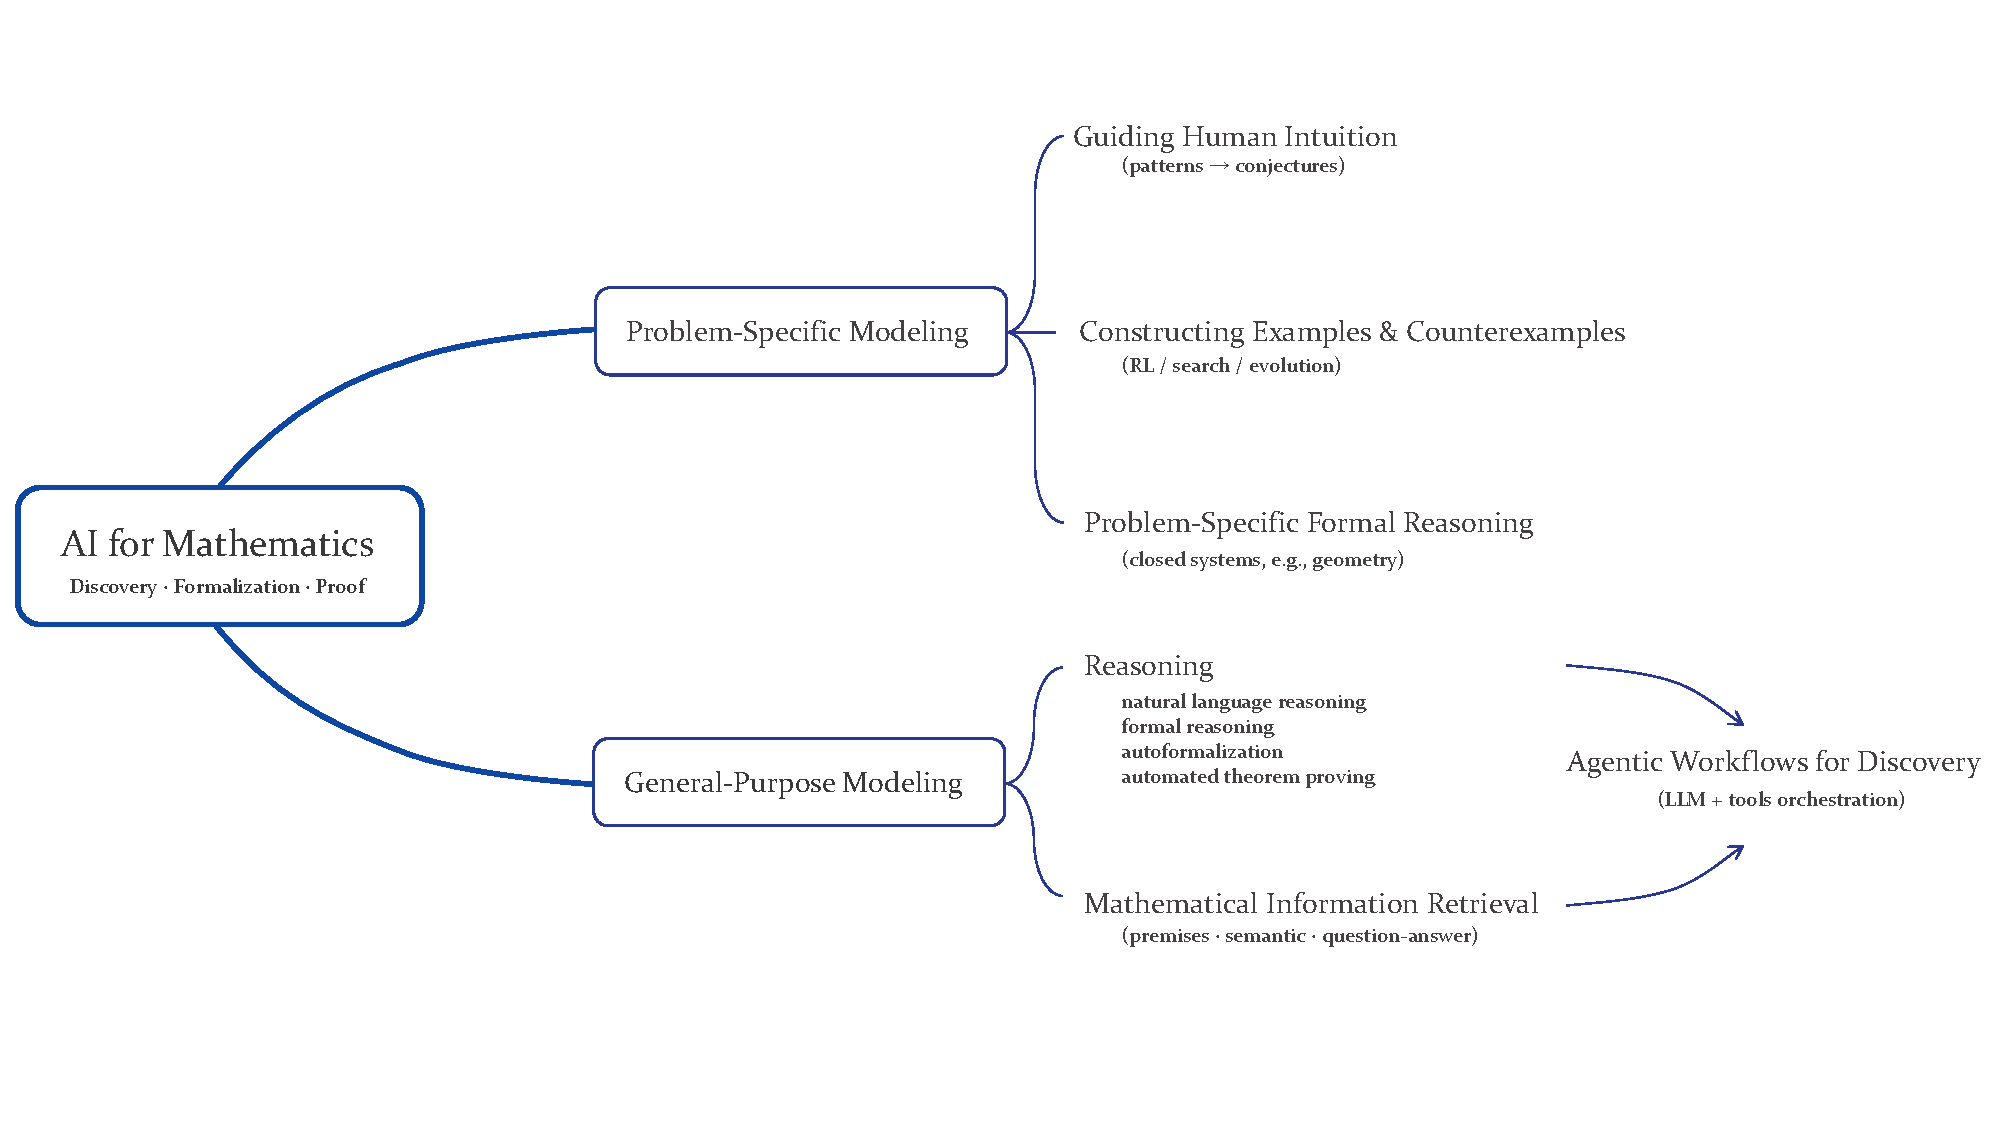
\includegraphics[width=0.95\linewidth]{figs/landscape.pdf}
\caption{AI4Math 研究方向的景观。AI4Math 研究可以大致分为两个互补的范式：\textit{特定问题建模}和\textit{通用建模}。特定问题建模包含三个主要工作方向：使用机器学习指导人类直觉、构建例子和反例，以及在封闭系统中执行形式推理。通用建模侧重于数学推理和数学信息检索；这些能力共同构成了新兴的数学发现代理工作流的基础。此图旨在组织和阐明研究方向之间的概念关系，而不是与本综述的各节提供一对一的对应关系。}
\label{fig:landscape}
\end{figure}


\section{特定问题建模}\label{sec:psm}
随着数据驱动技术的快速发展，研究人员开始设计针对特定数学研究问题量身定制的专用机器学习模型。这些努力通常分为三个不同的方向：识别高维数据中的模式以指导人类直觉并激发新的猜想；构建例子或反例以严格测试或反驳数学假设；以及在封闭的公理系统（如欧几里得几何）中执行形式推理。在本节中，我们回顾了这三个领域的最新发展，并讨论了它们各自的优势和局限性。


\subsection{通过机器学习指导人类直觉}

利用机器学习协助形成数学猜想的最早例子之一是 \cite{carifio2017machine}。在这项研究中，作者采用线性回归预测了一大组 F-理论几何中几何规范群的秩，成功地重新发现了一个关于规范群秩的现有猜想。在此基础上，他们将逻辑回归应用于涉及 $E_6$ 规范群的分类问题；通过对模型的归因分析，他们提出了一个全新的猜想，随后被人类数学家证明。

然而，证明深度学习在数学研究中广泛潜力的关键研究是 \cite{davies2021advancing}。这项工作的核心贡献是一个系统的框架，旨在加速猜想的生成过程——传统上，这是一个耗时的循环，数学家在其中假设关系，尝试证明并迭代地完善他们的想法。在 \cite{davies2021advancing} 提出的工作流中，数学家首先假设两个数学对象之间可能存在关系。然后训练一个专门设计的神经网络，根据一个对象的特征预测另一个对象的数量。随后使用归因方法来识别最具影响力的输入分量，从而引导数学家走向更精确和完善的猜想。这个循环重复进行，直到形成一个有数学意义的陈述。利用这种方法，作者在纽结理论中发现了代数和几何不变量之间的新关系 \cite{davies2024signature}，并提出了对称群组合不变性猜想预测的候选算法 \cite{blundell2022towards}。

受此范式启发，\cite{dong2024machine} 设计了另一个 AI 引导直觉框架，用于研究\textit{仿射 Deligne--Lusztig 簇（ADLV）}。这项工作不仅独立地重新发现了算术几何中经典的虚维数公式，而且还建立了一个新颖的、精确的下界定理。通过提供填补重要理论空白的定量刻画，该结果证明了\textit{AI 引导直觉}在促进纯数学深层领域严格发现方面的有效性。

除了完善猜想之外，机器学习还被证明在发现全新的数学现象方面是有效的。一个值得注意的例子是 \cite{he2025murmurations}，作者将椭圆曲线表示为向量，并训练了一个逻辑回归分类器来区分不同秩的曲线。为了解释分类器的强劲表现，作者对向量表示进行了主成分分析（PCA）。在绘制了给定导子范围内固定秩的椭圆曲线的 Frobenius 迹的平均值后，他们揭示了一种令人惊讶的振荡模式，他们称之为“murmurations”。此后，这一现象成为了深入理论研究的主题 \cite{zubrilina2025murmurations,lee2025murmurations,bober2025murmurations}。越来越多的文献继续利用机器学习来发现或重新发现各个领域的关系 \cite{carifio2017machine,KLAEWER2019438,PhysRevD.103.126014,doi:10.1142/S0217751X25500976,PhysRevD.105.066002,Lee01052025,doi:10.1142/S2810939223500016,PhysRevD.110.046016,shalyt2024unsupervised,lanard2025algorithm,lee2025machines}。





\subsection{构建例子和反例}

利用机器学习构建例子和反例的开创性工作之一是 \cite{wagner2021constructions}。在这项研究中，作者将图编码为 0-1 序列，并应用强化学习中的深度交叉熵方法来搜索作为现有猜想反例的图构造。在此先例之后，强化学习已被用于各种结构问题。例如，\cite{berczi2023ml} 将广中平祐（Hironaka）博弈——代数几何中奇点消除的核心框架——建模为马尔可夫决策过程（MDP）。通过结合蒙特卡洛树搜索和深度 Q 网络，作者成功训练了一个代理，用平滑点替换奇点，实现了 du Val 奇点的近乎最优消除。类似地，\cite{shehper2025what} 研究了 \textit{Andrews--Curtis (AC)} 猜想。在首先采用经典搜索算法识别了 \textit{Miller--Schupp} 级数无限子族的 AC 平凡性，并在 \textit{Akbulut--Kirby} 级数中获得长度缩减之后，作者将一般问题表述为 MDP。他们在不同难度的问题实例上训练了一个 RL 代理，最终发现了经典搜索方法未能找到的平衡表示的两个新颖的 AC 平凡化。

除了 RL，各种各样的其他机器学习技术已被提议用于数学构造。\cite{alfarano2024global} 在合成数据上训练了一个 Transformer 模型来预测稳定动力系统的 Lyapunov 函数；然后将训练好的模型用于发现非多项式系统的新颖 Lyapunov 函数。在组合数学中，\cite{charton2024patternboost} 引入了一种迭代的\textit{自举}程序。该方法首先通过局部搜索算法生成候选构造，在得分最高的候选上训练神经网络，然后从网络中采样新的种子来初始化下一轮局部搜索。利用这种方法，作者成功地发现了一个有 30 年历史的猜想的反例。\cite{bérczi2026flowbasedextremalmathematicalstructure} 提出了一种用于连续几何优化问题的几何感知条件流匹配模型，将流积分与约束流形的投影交织在一起。该方法使用带有扰动的随机松弛来初始化训练集，训练具有几何惩罚的条件流匹配模型，并采用几何感知采样以及基于奖励指导的策略优化来通过局部搜索迭代细化配置。这种方法在诸如最大化半径之和的圆堆积和 Heilbronn 三角形问题中发现了达到或超过已知最佳结果的配置。此外，\cite{BERGLUND2024138504} 应用遗传算法生成维度 2 到 5 的自反多胞体，识别了维度 5 中的几个以前未知的多胞体。其他利用机器学习构建例子或反例的工作包括 \cite{chervov2025cayleypy, chervov2025machine, Gukov_2025,swirszcz2025advancing,douglas2025diffusion}。

随着 LLM 能力的不断增强，基于 LLM 的代理也得到了改进，最近的几项工作证明了它们在发现新数学构造方面的潜力。\textit{FunSearch} \cite{romera2024mathematical} 使用进化方法搜索生成所需构造的程序。对于具有明确定义评估器的问题，FunSearch 使用现成的 LLM 迭代地将得分低的候选程序进化为得分高的程序。这是通过维护一个大型、多样化的程序池并重复提示 LLM 改进早期候选程序来实现的。利用这种方法，FunSearch 发现了大型上限集（cap sets）的新构造，超越了极值组合学中以前已知的最佳结果。建立在这一系列工作的基础上，\textit{AlphaEvolve} \cite{novikov2025alphaevolve} 使用了更强的 LLM，并将进化过程扩展到整个代码文件而不是单个函数，同时还同时优化多个指标。AlphaEvolve 已经为几个问题产生了改进的构造，包括\textit{最小重叠问题}和 11 维中的\textit{接吻数问题}。受 AlphaEvolve 启发的开源实现包括 \textit{OpenEvolve} \cite{openevolve}、\textit{ShinkaEvolve} \cite{lange2025shinkaevolve} 和 \textit{DeepEvolve} \cite{liu2025scientific}。AlphaEvolve 风格的代理特别适合于寻找可以通过编写代码来处理并用定义良好的评分函数进行评估的数学问题中的新构造。



\subsection{特定问题的形式推理}

\textit{AlphaGeometry} \cite{trinh2024solving} 代表了一种解决奥林匹克级别的欧几里得几何问题的神经符号方法。它将符号几何推理引擎与旨在建议辅助构造的语言模型集成在一起。基于演绎数据库（DD）\cite{chou2000deductive}和代数规则（AR）的符号组件，穷尽地推导给定前提集的演绎闭包。由于纯符号演绎无法引入新的几何对象（复杂证明通常需要这种能力），该系统利用语言模型来提出有用的辅助点。为了克服人类证明数据的稀缺性，作者通过交替进行符号演绎和随机点插入，生成了一个大规模的合成证明图数据集，随后通过回溯提取最小证明。在推理过程中，系统在一个循环中运行：符号引擎扩展演绎闭包，模型提出高概率的辅助点，循环重复，直到得出目标结论。这种架构使 AlphaGeometry 能够显著优于基于启发式的系统，达到与 IMO 银牌获得者相媲美的表现。

它的继任者 \textit{AlphaGeometry2} \cite{chervonyi2025gold} 通过表达能力和效率的提高进一步推进了这一范式。形式几何语言被扩展为支持轨迹描述、线性几何关系和非构造性陈述，而底层的符号引擎被重新设计以获得更高的速度和鲁棒性。这些改进使得能够为语言模型生成更大、更多样化的合成训练集。此外，AlphaGeometry2 引入了一种新颖的搜索算法，即\textit{搜索树的共享知识集成 (SKEST)}，它并行执行多个搜索树。通过允许这些树交换发现的信息，SKEST 显着改善了辅助构造空间的探索。因此，AlphaGeometry2 在 IMO 级别的几何问题上取得了金牌表现。除了用于辅助点生成的神经方法外，诸如 \textit{HAGeo} \cite{duan2025gold} 等近期工作提出了一种纯启发式策略，该策略引入了具有有利几何特性的辅助构造，包括直线和圆的交点、中点和点反射，并且同样达到了金牌水平的表现。有关欧几里得几何问题求解的其他工作可以在 \cite{zhang2023formalgeo,he2024fgeo,zou2024fgeo,zhang2024fgeo,zhang2024proposing} 中找到。



\subsection{讨论}

本节讨论的方法，识别模式以指导直觉、构建反例以及在封闭系统中执行形式推理，各自提供了独特的优势，同时也提出了独特的挑战。

\textit{AI 引导直觉}范式是强大的，因为它使数学家能够发现高维数据中的模式，否则这些模式很难或耗时地手动检测，从而有效地缩小了探索性研究中的搜索空间。然而，这种方法并非普遍适用。它依赖于仔细的问题选择，因为目标问题必须允许生成足够大且具有代表性的数据集。此外，成功的实施需要双重专业知识的高门槛：除了架构设计和损失工程等标准机器学习考虑因素外，深刻的数学见解对于解释模型输出和将经验相关性转化为严格的数学理论也是不可或缺的。最终，由于最终的证明和验证通常由人类数学家进行，因此该工作流程中的自动化程度仍然有限。

相反，使用机器学习构建例子和反例可以通过发现违背人类直觉的对象来显着加速猜想的提出和测试。然而，这个方向也面临着技术障碍，特别是在分布外 (OOD) 泛化方面。例如，\cite{alfarano2024global} 中的反向生成方法（通过从采样的解构造问题）可能会产生具有特定分布的训练集。这可能给泛化到典型问题实例带来挑战，并且通常需要精心设计的程序，例如作者提出的 Lyapunov 函数的多样性促进机制，以确保鲁棒的性能。此外，当采用 RL 时，将数学问题映射到 MDP 是不平凡的。定义适当的状态表示、动作空间和奖励函数可能会很复杂 \cite{wagner2021constructions}，而且稀疏奖励和长规划范围可能会使学习过程进一步复杂化 \cite{shehper2025what}。

像 FunSearch 和 AlphaEvolve 这样的系统代表了通过程序进化实现自动数学发现的强大转变。这些代理在构造类型的问题（例如在组合学中寻找极值配置或改进算法界限）中表现出色，在这些问题中，可以通过迭代优化代码来导航搜索空间，并通过明确定义的评分函数进行验证。然而，这种范式仍然固有地受到其对这种评估器的依赖的约束。虽然在识别特定的数学对象（例如上限集或高维球堆积）方面非常有效，但这些系统并未明确参与概念框架或结构原则的制定，而这些框架或原则是通用理论的基础或连接不同的数学领域。因此，它们的成功目前集中在可验证的构造上，将可转移的抽象和统一见解的发现留作一个开放的前沿。

最后，特定问题的形式推理系统，如 AlphaGeometry，证明了将符号引擎与神经语言模型相结合可以在结构化领域中实现专家级的性能。然而，这些系统的成功通常依赖于特定领域符号引擎的可用性（例如，用于几何的演绎数据库 \cite{chou2000deductive}）和生成大规模合成数据的能力。因此，这些架构通常与其特定的问题范围紧密相连，并且如果不进行大量修改，可能无法转移到数学的其他领域。

\section{通用建模}\label{sec:grm}

通用建模标志着从为孤立问题设计的专用算法向能够处理广泛数学领域的适应性系统的转变。与特定问题建模需要为每个新任务定制特征和架构不同，通用方法利用在海量语料库上训练的基础模型来学习数学知识的普遍表示。这些模型旨在支持广泛的活动，从解决各种问题集到检索定理和编排复杂的工作流，而无需针对每个新领域进行大量修改。

我们将通用建模的最新进展分为三个互补的方向：利用语言直觉能力的自然语言推理模型；通过与证明助手交互确保严谨性的形式推理模型；以及将推理建立在既定知识基础上的数学信息检索系统。本节首先分析基础模型（尤其是 LLM）的能力和固有的局限性，为我们详细回顾这三个关键领域确立背景。

\subsection{基础模型与 LLM}

与针对单个狭义定义任务进行训练的传统机器学习模型相比，LLM 充当基础模型：单个架构以统一的方式在广泛的数据集和任务上进行训练。在数学上，这种区别代表了从函数逼近到算子逼近的范式转变，这一过程与\textit{元学习}密切相关。传统模型通常旨在逼近欧几里得空间之间特定的、固定的映射 $f: \mathcal{X} \to \mathcal{Y}$，例如对图像中的对象进行分类，方法是插值从该特定流形采样的离散数据点。

相比之下，基础模型执行\textit{任务插值}而不是简单的数据插值。它们在海量任务分布 $\{T_i\}$ 上进行训练，其中每个任务有效地定义了不同的映射 $f_i$。通过学习在整个分布上泛化，基础模型不仅仅是逼近单个函数；相反，它逼近了一个作用于函数空间的全局算子（或泛函） $\Psi$。给定任务规范或上下文作为输入，$\Psi$ 实例化该上下文所需的特定映射 $f_i$。从本质上讲，传统机器学习逼近函数，而基础模型逼近生成和操作这些函数的算子。

它们成功的关键因素是处理多种数据类型的能力；标记化（tokenization）将异构输入转换为通用序列表示，并且下一个标记预测目标提供了统一适用于模型遇到的所有任务的单一学习规则。基于注意力的架构在这种机制中至关重要。除了随着模型大小和数据量有效扩展之外，注意力机制通过在训练期间加强长上下文连贯性，成为推理的关键引擎。这使得模型能够在扩展序列上捕获和维护复杂的依赖关系——逻辑演绎的先决条件。通过接触不同领域和监督信号，模型被迫将大量异构数据压缩为共享的内部表示，并发现跨任务和语言的通用低维结构。一个自然的假设是，这种低维结构的一个关键组成部分对应于可以用不同语言和领域表达的通用推理能力。

数学自然地融入了这个框架。数学工作受严格的逻辑规则支配，许多数学任务可以表述为在计算、推导或证明中产生下一个有意义的步骤——正是下一个标记预测目标旨在建模的那种逐步结构。因此，当在一个包含丰富数学和科学语料库的基础上训练 LLM 作为基础模型时，支持跨领域泛化和长上下文连贯性的相同机制可以被用来学习和使用广泛的数学推理能力。

然而，掌握标准化考试与从事研究级数学之间仍然存在根本差距。虽然当前模型在解决定义明确的本科问题方面表现出色，但研究需要开放式探索、绝对逻辑严谨性，以及驾驭专业领域知识“长尾”的能力——在这些挑战中，随机文本生成通常会失败。因此，为了将 AI 从称职的求解器提升为可靠的研究伙伴，通用建模必须超越简单的下一个标记预测，整合形式验证、语义检索和代理工作流，以弥合看似合理的文本与严谨真理之间的鸿沟。

\subsection{自然语言推理}\label{subsec:nlr}

当前自然语言数学推理的方法通常分为两类：\textit{数学专用 LLM} 和 \textit{通用推理模型}。

数学专用 LLM 通常通过专门的预训练和后训练管道从通用基础模型调整而来。在预训练期间，过滤管道 \cite{shao2024deepseekmath,yang2024qwen2} 从网络语料库（例如 Common Crawl）、教科书和研究论文中提取高质量的数学内容，以最大化领域相关性。后训练使用监督微调（SFT）和强化学习（RL）改进这些模型。SFT 的数据通常构造为思维链（CoT）\cite{wei2022chain} 对，由问题和分步解决方案组成，或结合了外部代码执行的工具集成推理（TIR）\cite{goutora} 示例。一个突出的例子是 \textit{NuminaMath} \cite{li2024numinamath}，它通过在高质量 CoT 和 TIR 数据集上微调赢得了首届 AIMO 进展奖。虽然这一类别的模型 \cite{azerbayev2024llemma,shao2024deepseekmath,yang2024qwen2,ying2024internlm} 在小学和竞赛级基准（例如 GSM8K \cite{cobbe2021training}、MATH \cite{hendrycksmath2021}、AIME）上表现出色，但它们在高等数学方面的能力探索较少。

与此同时，通用 LLM 通过规模和新颖的推理策略取得了重要的数学里程碑。像 GPT-3 这样的早期迭代在基本算术方面遇到了困难，而 GPT-4 \cite{achiam2023gpt} 在 GSM8K 上达到了 92.0\%。随着\textit{测试时缩放}（test-time scaling）的引入，范式发生了转变，模型在推理期间将更多的计算投入到推理中。OpenAI 的 o1 模型在 AIME 上展示了强劲的表现，随后的推理模型 \cite{guo2025deepseek,qwq32b,yang2025qwen3,comanici2025gemini} 进一步验证了这一方法。到 2025 年，增强推理模型（例如 Google 的 Gemini Deep Think）完全使用自然语言推理在国际数学奥林匹克（IMO）中达到了金牌表现，标志着该技术在高中奥林匹克数学领域已完全成熟。

然而，从奥林匹克问题过渡到高等数学面临着更严峻的挑战。先前的研究表明，虽然 GPT-4 可以协助处理本科主题，但它需要关键的人工监督 \cite{collins2024evaluating}，并且通常在研究生水平上失败 \cite{NEURIPS2023_58168e8a}。最近的基准量化了这一差距：\cite{jiang2025fate} 报告说，DeepSeek-R1 在研究生代数（FATE-H）上实现了 71.0\% 的证明准确率，但在博士资格考试（FATE-X）上降至 33.0\%。类似地，在 \textit{FrontierMath} 基准 \cite{glazer2024frontiermath}（由未发表的研究级问题组成）上，Gemini 3 Pro 在研究级拆分（第 4 层）\footnote{\href{https://epoch.ai/frontiermath}{https://epoch.ai/frontiermath}} 上得分为 18.75\%，这表明强大的研究级推理仍然是一个未解决的问题。

为了实证评估最先进模型的当前能力，我们构建了一个包含 100 个问题的数据集，这些问题取自北京大学（PKU）11 门本科数学科目的期末考试。我们评估了五个模型：GPT-4、o1、o3-mini、DeepSeek-R1 和 Gemini 2.5 Pro。示例问题和模型响应在附录 \ref{sec:exam} 中提供。人类专家以 0-5 分制对输出进行评分（标准见表 \ref{tab:score_crtr}）；归一化结果如 图 \ref{fig:nl_reason}（左和中）所示。虽然 GPT-4 得分低于 60，但推理增强模型（OpenAI o-系列、DeepSeek-R1、Gemini 2.5 Pro）显示出显着改进，其中几个得分超过 90。

此外，我们在北京大学的分析、概率、代数和几何与拓扑博士资格考试的 58 个问题上评估了 o3-mini。如图 \ref{fig:nl_reason}（右）所示，o3-mini 的平均得分为 84.4。仔细检查各个科目的表现发现了一个显著的差异：该模型在代数方面表现出最强的熟练程度，而在几何与拓扑方面得分最低。在假设这些考试对人类学生构成可比挑战的前提下，这表明当前的 AI 系统相对更擅长处理抽象代数结构，而不是需要几何直觉的任务。虽然由于潜在的数据污染以及与开放研究相比考试问题的特定性质，必须谨慎解释这些结果，但它们提供了强有力的证据，证明顶级模型现在可以处理大部分研究生级数学。

综合这些发现，我们观察到一个清晰的轨迹：LLM 的数学推理能力已从掌握基本计算和高中竞赛发展到精通本科课程，并且现在开始渗透到研究生和研究级数学领域 \cite{bryan2026motivic,jang2025point}。

\begin{figure}[tb]
\centering
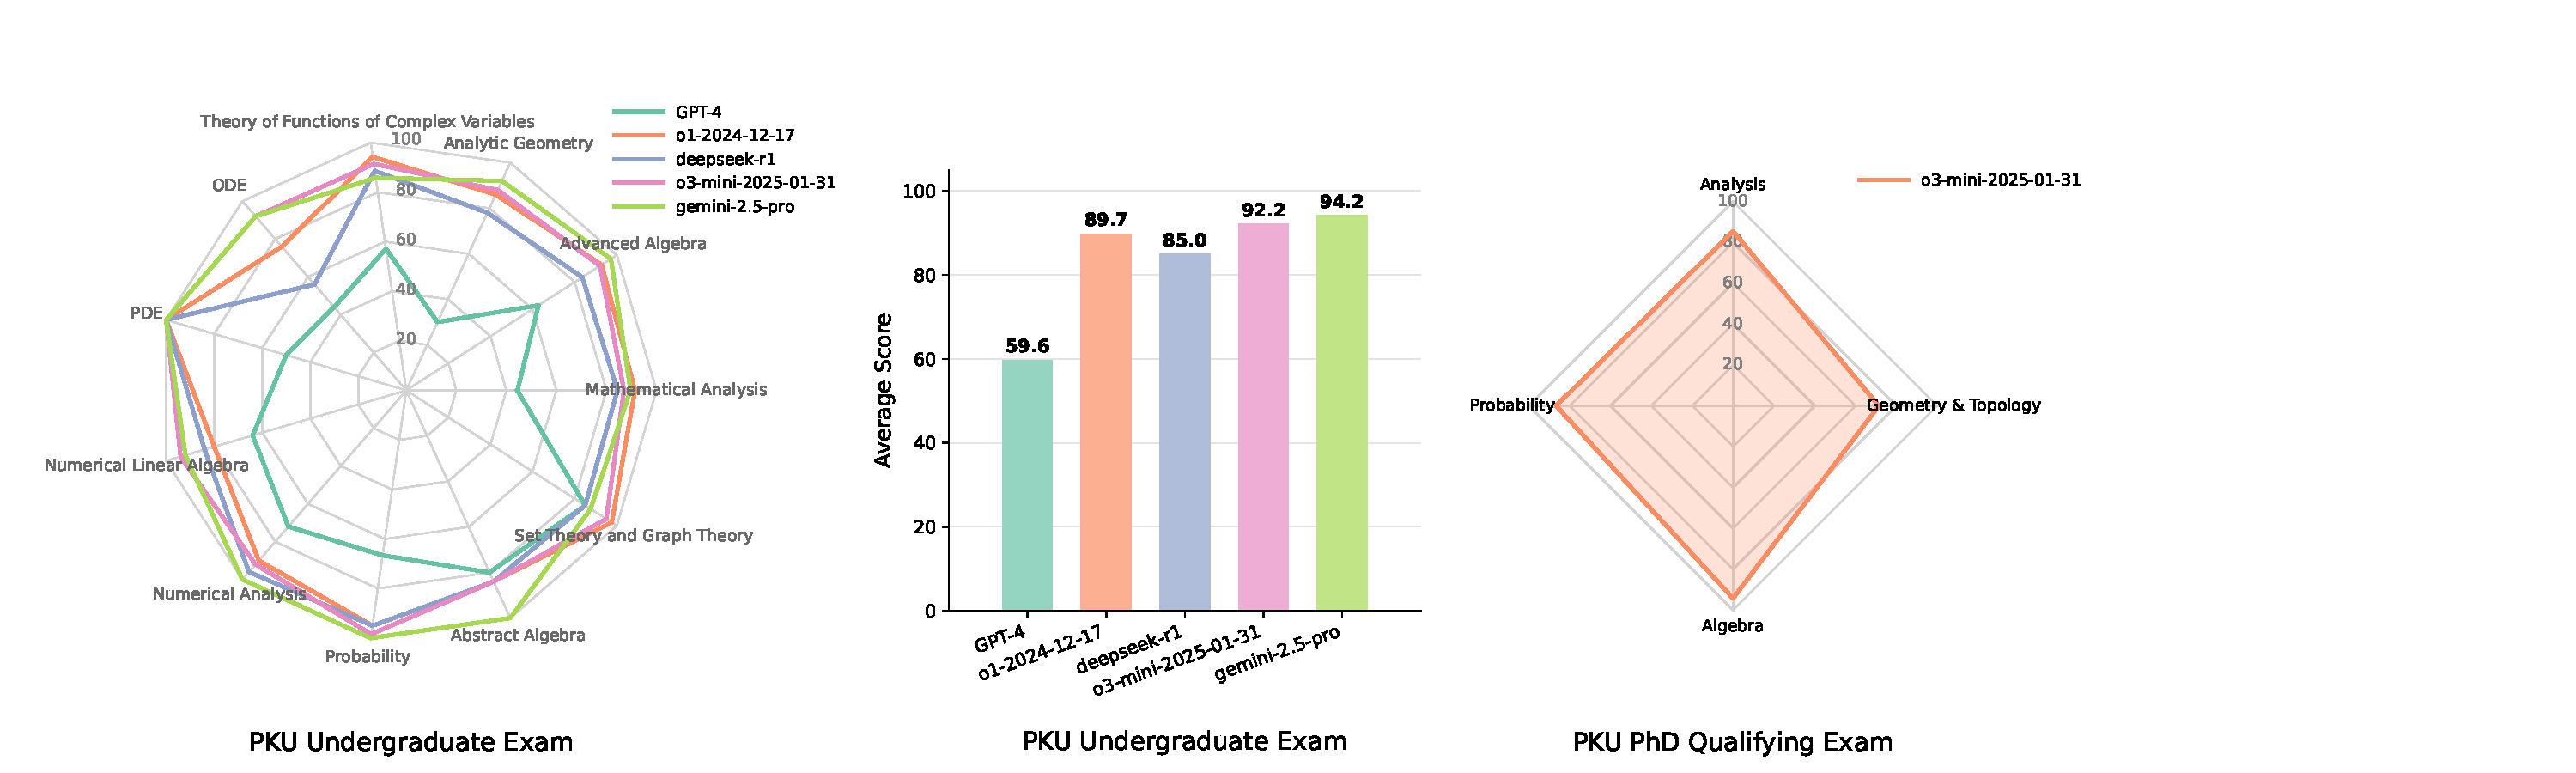
\includegraphics[width=0.95\linewidth]{figs/nl_reason.pdf}
\caption{五个 LLM 在北京大学 (PKU) 不同考试中的表现。左图：11 门本科科目的得分。中图：五个 LLM 在这些科目上的平均得分。右图：o3-mini 在四个博士资格考试领域的表现（平均得分：84.4）。}
\label{fig:nl_reason}
\end{figure}

\subsection{形式推理}\label{subsec:fr}

尽管顶级 LLM 现在可以解决某些研究生级甚至某些研究级问题，但评估它们的能力仍然是一个涉及大量人力的重大瓶颈。随着数学复杂性的增加，评估严重依赖领域专家；然而，由于自然语言固有的不精确性，即使是经验丰富的数学家也可能误判论证。一个著名的历史例子发生在 1994 年，当时发表在《数学年刊》（\textit{Annals of Mathematics}）上的一项结果声称，Busemann-Petty 问题在至少四维中具有负面解决方案 \cite{zhang1994intersection}。这一结论后来被证明是不正确的 \cite{koldobsky1998intersection,koldobsky1998advances}，并且 1999 年的一篇论文确立了该问题在四维中实际上具有正面解决方案 \cite{zhang1999positive}。类似地，2004 年发表在《数学年刊》上的一篇论文 \cite{schumacher2004quasi} 在 2006 年发现其主要结果的反例后，于 2023 年被撤回 \cite{schumacher2023retraction}，该反例被确定 \cite{kollar2006non}。这些案例表明，即使在顶级期刊严格的同行评审过程中，错误也可能持续存在。因此，为了实现快速可靠的数学推理验证，研究必须走向更加机械和明确的框架。形式系统正好提供了这样一个基础。在本节中，我们讨论形式系统对数学研究的好处及其在增强 LLM 推理能力方面的效用，然后回顾自动定理证明和自动形式化的最新进展。

\subsubsection{形式系统}

形式系统提供了一种精确的符号语言，配以严格定义的构建和验证证明的机制。存在各种系统，它们的区别在于底层的逻辑基础：HOL 系统（如 HOL Light、Isabelle/HOL）使用简单类型论；Coq（现在称为 Rocq）和 Lean 采用依赖类型论；Metamath 运行在一阶逻辑上，具有明确指定的公理；Mizar 建立在 Tarski-Grothendieck 集合论的基础之上。一旦数学论证被翻译成交互式定理证明器（ITP）的形式语言，就可以以绝对的严谨性对其进行验证。如果 1994 年关于 Busemann-Petty 问题的错误结果在这样的系统中被形式化，那么底层的逻辑缺陷很可能会被立即发现，从而防止错误主张的发表。

除了其对数学正确性的内在价值之外，形式系统还为 AI 开发提供了一个关键优势：它们提供可靠的、可验证的监督。与基本数学（答案通常是数字的并且容易检查）不同，高级的以证明为导向的问题缺乏简单的验证器，这使得很难产生可靠的训练信号。交互式定理证明器通过提供关于每个逻辑步骤有效性的精确反馈来弥补这一差距。此功能为强化学习提供了高质量的训练信号，从而使模型能够在严谨的设置中发展出更强的推理能力。

在交互式定理证明器中，Lean \cite{DBLP:conf/cade/MouraKADR15,DBLP:conf/cade/Moura021} 培育了一个特别强大的生态系统。其统一的数学库 \textit{mathlib4} 通过大规模的社区协作而迅速扩展，截至 2025 年 12 月，包含超过 250,000 个定理和 120,000 个定义。该领域的一个里程碑式成就是 \textit{Liquid Tensor Experiment}，由 Johan Commelin 领导，它形式化了 Peter Scholze 关于液态向量空间的一个中心定理。最初对证明的正确性持怀疑态度的 Scholze 评论说，该定理可能是他“迄今为止最重要的定理”\footnote{\href{https://xenaproject.wordpress.com/2020/12/05/liquid-tensor-experiment/}{https://xenaproject.wordpress.com/2020/12/05/liquid-tensor-experiment/}}。该项目历时约 18 个月，不仅验证了结果，还简化了原始的 Clausen-Scholze 证明，帮助 Scholze 加深了他对论证结构的理解\footnote{\href{https://xenaproject.wordpress.com/2021/06/05/half-a-year-of-the-liquid-tensor-experiment-amazing-developments/}{https://xenaproject.wordpress.com/2021/06/05/half-a-year-of-the-liquid-tensor-experiment-amazing-developments/}}。此外，Liquid Tensor Experiment 促进了 mathlib4 中代数基础设施的开发：它推动了同调代数和范畴论的早期形式化，并吸引了一批代数学家加入社区。其他值得注意的里程碑包括多项式 Freiman-Ruzsa (PFR) 猜想的形式化\footnote{\href{https://teorth.github.io/pfr//}{https://teorth.github.io/pfr//}}、球面外翻定理\footnote{\href{https://leanprover-community.github.io/sphere-eversion/}{https://leanprover-community.github.io/sphere-eversion/}}，以及正在进行的关于形式化 8 维球堆积问题解的工作。

然而，这些项目仍然是劳动密集型的，需要专家手动将定义和证明转化为代码。这种高成本促使开发 \textbf{自动形式化} 工具和 \textbf{自动定理证明器}，以加速数学知识的\textit{数字化}——将标准的非形式数学转化为诸如 Lean 这样的严谨形式系统。

\subsubsection{自动形式化}

自动形式化是指以自主方式（例如通过语言模型）将自然语言的数学陈述和证明翻译为形式代码的任务。该领域的早期工作采用了在对齐数据上训练的序列到序列模型。例如，\cite{wang2018first} 通过非形式化 Mizar 陈述构建数据集，以训练翻译模型。为了解决对齐对的稀缺问题，\cite{wang2020exploration} 随后探索了基于循环一致性损失的无监督方法，其中模型学习通过在非形式和形式域之间翻译陈述来重建陈述，而无需显式监督。

LLM 的出现从根本上改变了这种范式。研究表明，现成的 LLM 可以通过少样本提示生成合理的形式化 \cite{wu2022autoformalization,gadgil2022towards,agrawal2022towards,azerbayev2023proofnet}。关键的是，\cite{wu2022autoformalization} 观察到一种不对称性：将形式代码翻译成自然语言（非形式化）对于模型来说比反向操作容易得多。这一见解促进了大规模合成数据集的创建，在这些数据集中，使用 LLM 将海量形式库（如 mathlib4）非形式化，以生成高质量的对齐对，用于训练专门的自动形式化器 \cite{jiang2023multilingual,lu2024process,gao2025herald,liu2025rethinking}。

最近的工作侧重于提高这些系统的质量和接地（grounding）。\textit{Herald} \cite{gao2025herald} 引入了一种尊崇库 mathlib 依赖图的层次非形式化策略。通过按拓扑顺序翻译声明，它确保在翻译相关的定理时，先决条件概念的自然语言描述是可用的。Herald 进一步通过基于策略的状态合成来扩充其数据，并在 miniF2F 验证集上实现了超过 96\% 的陈述自动形式化准确率。为了增强接地，\textit{RAutoformalizer} \cite{liu2025rethinking} 采用检索机制将生成的代码锚定在现有的形式声明中。针对研究级数学中常见的概念缺失挑战，\cite{wang2025aria} 提出了 \textit{Aria}，一个基于 LLM 的代理系统。更一般地说，基于 LLM 的代理是指通过与其环境的显式交互循环运行的系统：它维护中间状态，对观察结果进行推理，执行多步规划并相应地选择动作。这些动作可能包括调用外部工具，例如语义检索、符号推理模块或代码合成组件，并使用来自环境的反馈来指导后续决策。这种代理设计使得复杂的任务能够被分解为结构化的子任务，并支持超越单次传递生成的迭代细化 \cite{wang2024survey}。在此框架内，Aria 将非形式陈述分解为概念的依赖图；如果 mathlib 库中缺少某个概念，代理将使用语义搜索和合成自下而上地递归定义它，从而有效地处理数学词汇的“长尾”。

\paragraph{评估与验证}
评估陈述的自动形式化是不平凡的。一旦陈述被正确自动形式化，由于形式系统的存在，评估自动形式化的证明就变得简单直接，这使得陈述自动形式化成为从评估角度来看的主要困难。虽然人类专家审查是黄金标准，但它是不可扩展的。因此，挑战在于开发正确性的自动化指标。
\begin{itemize}
    \item \textbf{有基准真相时：} 当存在参考形式陈述时，可以通过逻辑等价性而不是仅仅通过字符串匹配来评估正确性。例如，\textit{BEq} \cite{liu2025rethinking} 利用神经定理证明器来检查生成的陈述和基准真相是否可以相互推导。在 \cite{liu2025assess,poiroux2025reliable} 中探索了类似的等价检查方法。

    \item \textbf{无基准真相时（语义验证）：} 在没有参考的情况下，必须验证\textit{语义正确性}——形式代码是否忠实地捕捉了非形式陈述的意图。一种朴素的方法涉及“回译”，即 LLM 将代码翻译回英语以进行比较 \cite{ying2024lean,gao2025herald}。然而，由于 LLM 可能会错过细微的逻辑差异，这很容易出错。为了减轻这种情况，\cite{xuejun2025mathesis} 提出了 \textit{Mathesis}，一个细粒度的评估框架。Mathesis 将陈述分解为假设和结论，分别评估每个组件的对齐情况，并使用模糊积分聚合这些分数以严格拒绝不一致。为了进一步协助验证，Aria \cite{wang2025aria} 通过检索形式陈述中每个术语的详细元数据（类型、值、非形式描述）来丰富上下文，从而实现更准确的语义判断。
\end{itemize}
可靠的验证器不仅对评估至关重要，而且还作为强化学习的关键奖励模型，创建一个迭代改进自动形式化性能的反馈循环 \cite{xuejun2025mathesis,lu2024process,huang2025formarl}。

\textit{注：} 本节重点讨论\textit{陈述}的自动形式化。\textit{证明}的自动形式化（需要翻译逻辑推理步骤而不仅仅是定义）与自动定理证明密不可分。因此，我们在下一节的证明生成背景下讨论证明的自动形式化。

\subsubsection{自动定理证明}

\begin{figure}[tb]
\centering
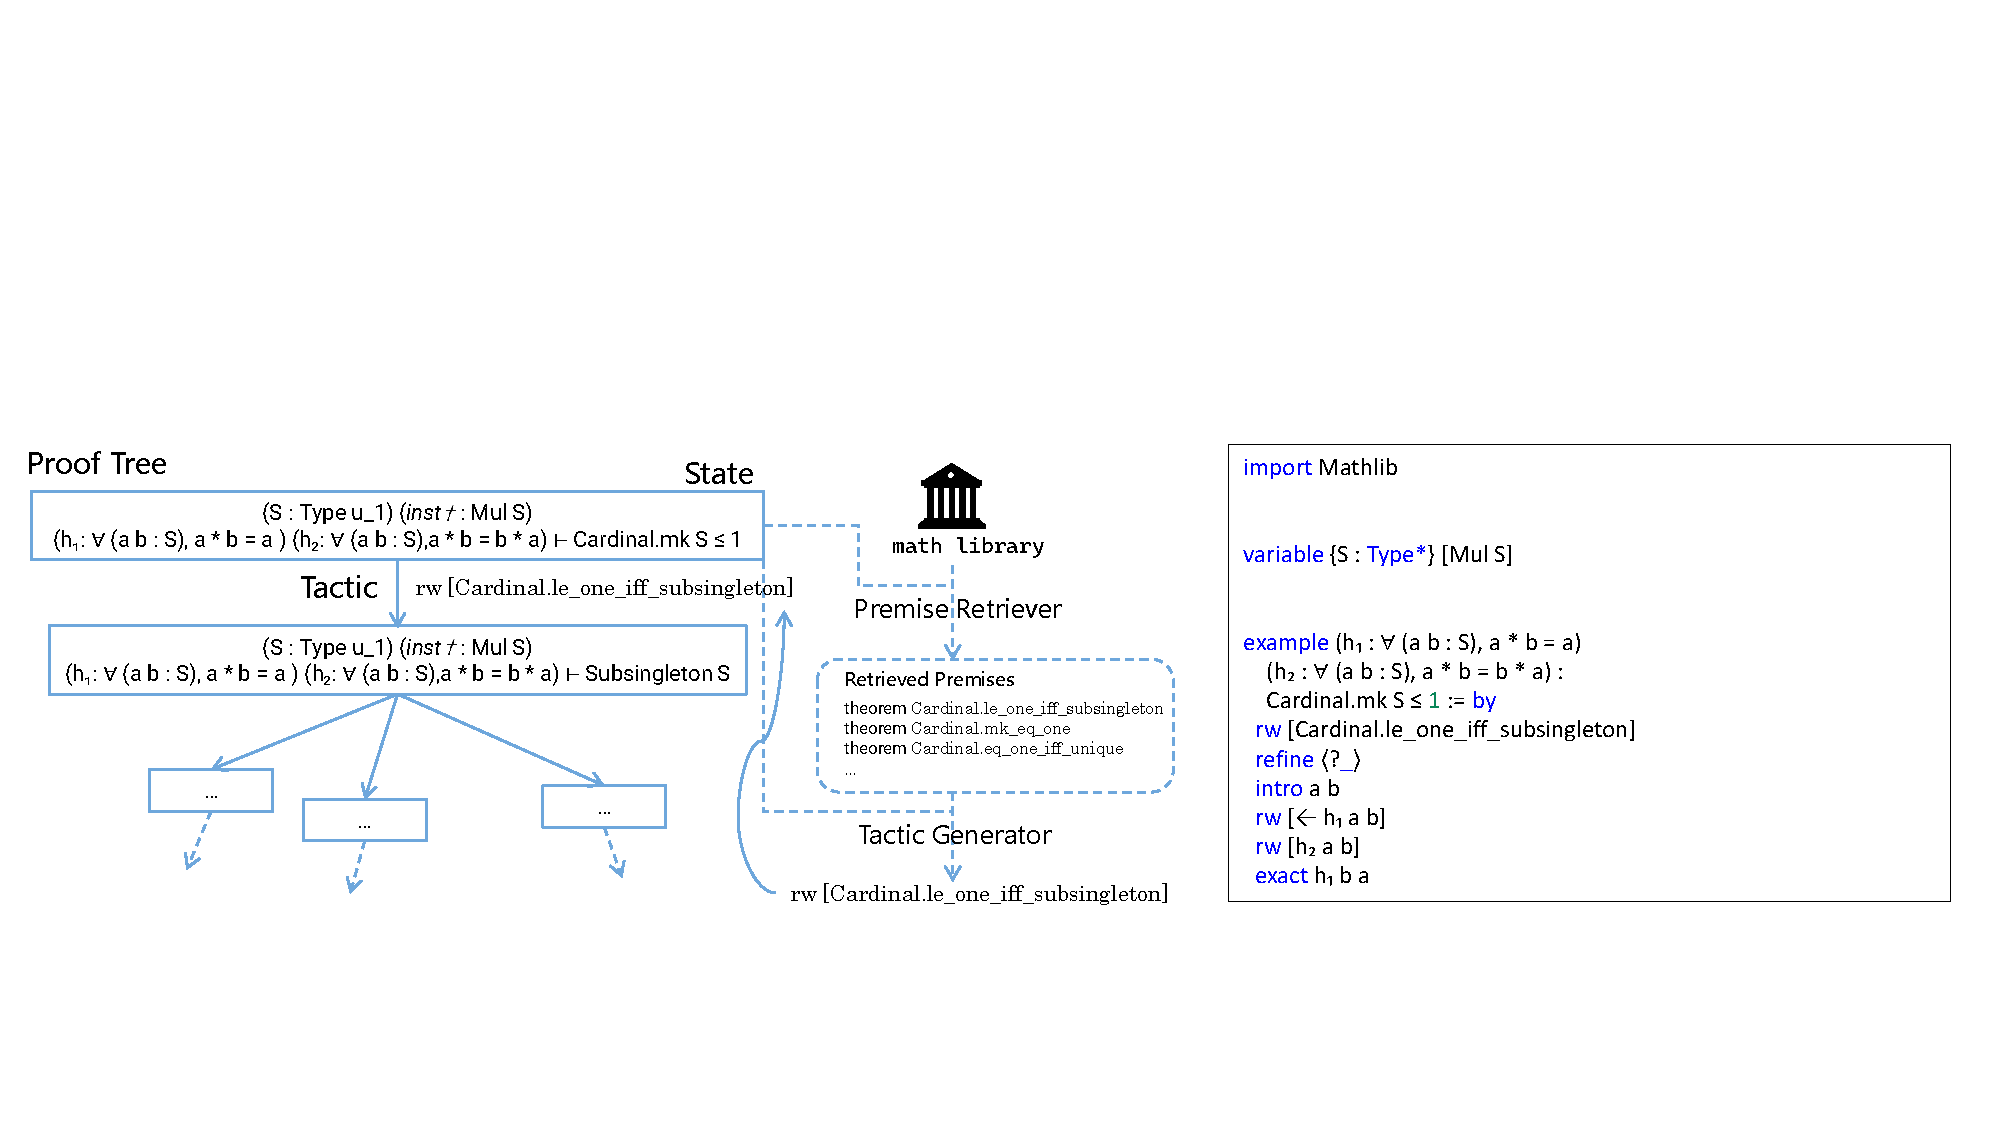
\includegraphics[width=0.95\linewidth]{figs/proof-tree.pdf}
\caption{证明步骤生成方法的示例及其生成的完整证明。左图：证明树的图解，其中每个节点表示一个证明状态，每条边对应一个策略（tactic）。应用适当的策略将当前的证明状态转换为下一个状态。在每一步中，证明步骤生成方法检索相关前提并提出几个候选策略进行尝试。右图：此过程最终获得的完整证明。}
\label{fig:proof-tree}
\end{figure}

形式系统中的自动定理证明旨在为形式陈述生成有效的证明。基于深度学习的解决此任务的方法分为两大类：\textit{单模型方法} 和 \textit{代理方法}。单模型方法可进一步分为\textit{证明步骤生成}和\textit{整个证明生成}方法。

\paragraph{证明步骤生成}
证明步骤生成方法将定理证明表述为树搜索问题。在这个框架中，搜索树中的每个节点对应一个证明状态，每个动作对应一个策略的应用，该策略将证明器转换到一个新的证明状态。一旦找到通向没有剩余目标的路径，就成功构建了证明。图 \ref{fig:proof-tree} 演示了由这种方法产生的证明树的示例，以及最终证明。

证明步骤生成的优势在于\textit{可重用性}和\textit{探索}。在搜索过程中，证明状态是可重用的：如果新遇到的状态与先前探索的状态重合，它们可以被合并。此外，该系统通过在每一步尝试多种策略，展现出强大的探索能力。然而，由于树搜索的计算成本，这些方法通常面临推理速度慢的问题，训练稳定性困难，并且在训练和推理过程中严重依赖于高效的交互工具。

该领域最早的神经方法之一是 \textit{Holophrasm} \cite{whalen2016holophrasm}，它采用蒙特卡洛树搜索（MCTS）进行探索。Holophrasm 集成了三个神经组件：一个用于检索有用定理的\textit{相关性网络}，一个用于提出变量替换的\textit{生成网络}，以及一个用于估计可证明性的\textit{价值网络}。随后的工作主要将策略预测视为分类问题，代表性例子包括 \textit{GamePad} \cite{huang2018gamepad}、\textit{DeepHOL} \cite{bansal2019holist} 和基于图的方法 \cite{paliwal2020graph}。超越纯分类，\textit{GPT-f} \cite{polu2020generative} 通过条件语言建模目标训练 Transformer 生成证明步骤，并使用最佳优先搜索构建证明。类似地，\cite{lample2022hypertree} 引入了一种基于超树的搜索，结合了在线训练策略，其中策略和评价模型在从重复的证明搜索中收集的数据上定期更新。

这一领域的主要挑战是缺乏大规模形式数据。为了缓解这一瓶颈，研究人员追求了两个互补的方向：在有限的形式数据下提高模型性能，以及合成额外的形式数据。对于前者，\textit{ABEL} \cite{gloeckle2024abel} 提出了一个具有优先采样的在线强化学习框架以鼓励探索；值得注意的是，其 RL 阶段仅在 244 个形式陈述上进行了训练，却达到了与当时最先进水平相当的表现。对于后者，\textit{REAL-Prover} \cite{shen2025real} 提出了一个集成管道，包括用于翻译非形式陈述的陈述自动形式化器、在相关前提条件为条件下生成策略的检索增强证明器，以及\textit{专家迭代}范式。在这个循环中，模型在生成的状态-策略对上进行训练，执行证明搜索，并迭代地从成功的搜索中收集新的训练数据。建立在 REAL-Prover 检索增强架构的基础上，作者引入了 \textit{reap} \footnote{\href{https://github.com/frenzymath/reap}{https://github.com/frenzymath/reap}} 策略，作为检索引导的证明自动化的具体实例化。reap 策略目前处于 Beta 测试阶段，并作为 mathlib4 的候选功能分支进行维护。

一个值得注意的里程碑是 \textit{AlphaProof} \cite{hubert2025olympiad}。AlphaProof 训练了一个 3B 参数的证明网络，共同输出策略和价值估计。其训练管道包括对 300B 令牌的预训练，对 300k 状态-策略对的监督微调，以及对 8000 万个自动形式化陈述的强化学习。这些形式陈述源自大约 100 万个非形式问题，其中自动形式化模型在（非形式陈述，形式化思维链，形式陈述）的三元组上进行训练，每个问题生成多个不同的翻译。对于特别具有挑战性的任务，AlphaProof 应用\textit{测试时强化学习}，通过构建和训练专门的课程来适应问题结构。因此，它取得了与 IMO 银牌获得者相媲美的表现。其他值得注意的方法包括 \cite{jiang2022thor, polu2023formal, wang-etal-2023-dt, yang2023leandojo, xin2025bfs, li2024hunyuanprover,xin2025scaling}。

\paragraph{整个证明生成}
相比之下，整个证明生成方法旨在一次前向传递中生成整个形式证明，并可能包含内联注释。它们的主要优点是推理速度快且在生成过程中独立于交互工具。然而，与逐步搜索相比，它们的探索能力有限；它们通常依赖行为克隆，并且更容易出现错误累积，因为它们无法访问中间的证明状态。

这种范式在很大程度上依赖于数据的质量和数量。由于没有确定数据质量的先验方法，通常通过模型性能进行间接评估。为了解决数据数量问题，\cite{xin2024deepseek} 提出了一个集成的管道，包括自动陈述形式化、过滤（以移除琐碎或错误的陈述）、陈述证明，以及在产生的经验证对上进行迭代训练。在此基础上，\textit{DeepSeek-Prover-V1.5} \cite{xin2025deepseekproverv} 通过构建更丰富的数据集（包括在形式代码之前编写的非形式证明和内联的非形式注释），并应用\textit{来自验证器反馈的强化学习（RLVF）}，提高了性能。采用这种范式的其他工作包括 \cite{first2023baldur, azerbayev2024llemma, ying2024internlm, dong2025stp, zhang2025leanabell,wang2025kimina,lin2025goedel}。

\paragraph{代理方法}
代理方法 \cite{jiang2023draft,wang2024legoprover,varambally2025hilbert,Chen_et_al_2025_Seed-Prover1.5,jiang2025fate,gloeckle2025reinforcement,achim2025aristotle} 代表了从单模型系统向模块化工作流的范式转变。这些方法将定理证明分解为协调的子任务，例如检索、分解和验证，这些子任务通过整合语言模型与外部工具的结构化工作流来编排。这些方法的有效性依赖于三个核心组成部分：强大的检索系统、LLM 的推理能力，以及旨在模仿数学研究过程的工作流。

\textit{草稿、草图和证明（DSP）} \cite{jiang2023draft} 是该范式的原型。它生成一个非形式证明，将其转换为具有开放子目标的形式草图，并使用轻量级证明器关闭它们。\textit{LEGO-Prover} \cite{wang2024legoprover} 通过维护一个持久的引理池来扩展它。独特的是，它通过\textit{维度扩展}、\textit{关键概念识别}、\textit{参数化}和\textit{复杂度增强}等策略，将已验证的引理演化为新的引理。\textit{Hilbert} \cite{varambally2025hilbert} 在定理检索的指导下，通过递归的子目标分解将非形式证明转换为形式草图。\textit{Seed-Prover-1.5} \cite{Chen_et_al_2025_Seed-Prover1.5} 同样采用了专门的草图模型和专用的证明模型，在研究生级基准 FATE-H 上实现了 80\% 的准确率，在博士级基准 FATE-X 上实现了 33\% 的准确率 \cite{jiang2025fate}。值得注意的是，对于诸如 Seed-Prover 之类的代理方法，广泛使用的 miniF2F 基准 \cite{zheng2021minif2f} 已经很大程度上饱和，可以被视为已有效解决。为了解决非形式推理和形式代码之间的粒度差距，\cite{wang2025translating} 提出了一个两阶段状态链（CoS）框架。通过在生成特定转换策略之前提取与非形式论证的逻辑流对齐的中间形式状态序列，这种方法在有限计算预算下显著降低了策略生成的复杂性。

像 \textit{Aristotle} \cite{achim2025aristotle} 这样的高级代理交替进行非形式推理和形式验证。Aristotle 将证明起草为引理序列，对其进行形式化并尝试验证，然后基于反馈迭代地完善其输出。结合几何求解器，它达到了 IMO 金牌水平的表现。\textit{Numina-Lean-Agent} \cite{liu2026numina} 为编码代理 Claude Code 配备了 Lean-LSP-MCP \cite{lean-lsp-mcp} 用于与 Lean 交互，一个用于定理检索的语义搜索引擎，一个非形式证明器 \cite{huang2025winning}，以及一个外部 LLM 用于额外的推理支持。它成功解决了 2025 年普特南竞赛中的所有问题，这是一项最初由 \textit{AxiomProver} \cite{axiommath_fromSeeingWhy_2025} 报告的成就。Numina-Lean-Agent 还在数学家的帮助下形式化了一篇关于 Brascamp-Lieb 不等式的研究论文 \cite{benard2025effective}，通过迭代细化表示为陈述和证明的依赖图的自然语言蓝图。\textit{Gauss} 代理 \cite{mathinc_gauss} 展示了人类-AI 协作的力量，它在专家支架（scaffolding）的帮助下，在三周内形式化了强素数定理。这些结果表明，精心设计的代理工作流可以有效地利用内在的推理能力和外部工具，在自动定理证明中实现显著的收益。

形式推理代理的实际影响，在最近特伦斯·陶（Terence Tao）探讨保罗·埃尔德什（Paul Erdős）猜想的工作中最能清晰体现\footnote{\href{https://github.com/teorth/erdosproblems/wiki/AI-contributions-to-Erd\%C5\%91s-problems}
     {https://github.com/teorth/erdosproblems/wiki/AI-contributions-to-Erd\%C5\%91s-problems}}。在 2025 年末至 2026 年初，像 Aristotle 这样的代理系统成为高杠杆验证管道中不可或缺的组件：前沿语言模型（例如 Gemini Deep Think，ChatGPT）被用于生成候选构造或启发式论证，然后将这些在 Lean 中进行严格形式化和机械验证。该管道已经产生了对几个埃尔德什问题（特别是问题 \#205）经过形式验证的反例，以及对更复杂问题（例如 \#367）的部分解答，同时许多相关情况仍未解决。重要的是，这些例子最好被视为具有代表性而不是结论性的：这个过程正在进行中，更多的结果还在不断出现。虽然形式化极大地降低了不可挽回的幻觉风险，但它并不能消除所有的失败模式——模型可能仍然会利用意外的问题规范或重新发现后来在文献中找到的论证。尽管如此，这些发展标志着一种定性的转变。形式推理代理现在可以充当可靠的研究副驾驶，系统地将启发式洞察力转化为经过认证的数学知识，并缓解探索性数学中长期存在的验证瓶颈。

\subsection{数学信息检索}\label{subsec:mir}

数学信息检索涉及从大量数学文档集中检索数学内容（包括公式、定理和问题解答）的任务。与标准文本检索相比，MIR 必须明确考虑数学表达式独特的结构和语义。数学公式本质上是结构化对象，其含义取决于符号组合和关系结构，而不仅仅是词汇重叠。因此，有效的 MIR 系统必须解决诸如匹配数学结构和符号模式等挑战，同时利用周围的文本上下文来解决歧义并解释含义。

关键的是，MIR 不仅仅是人类用户的搜索工具，而是现代自动定理证明（ATP）和 AI 代理系统的基本组件。在 ATP 的背景下，\textit{前提检索}——从庞大的库中识别有用的定理、引理或定义以证明新定理的任务——通常是主要的瓶颈。随着数学库的增长以包含数十万个形式陈述（例如 mathlib4），有效检索“大海捞针”的能力决定了证明器是能够解决问题还是超时。对于代理系统，MIR 使得能够访问长期数学记忆，允许代理将他们的推理建立在既定知识的基础上，而不是产生毫无根据的事实的幻觉。这需要从传统的基于关键字的匹配转向基于推理的检索。强大的 MIR 模型必须理解逻辑蕴含和数学等价性；例如，它必须认识到一个指出“方阵具有非零行列式”的定理是回答关于“矩阵的列是否形成线性独立集”的查询所需的关键前提，尽管这两个陈述之间没有共享关键字。

根据检索目标的粒度和查询的性质，MIR 包含几个密切相关的任务。突出的例子包括\textit{前提检索}、\textit{语义检索}和\textit{问答检索}。

\paragraph{前提检索}

在自动定理证明中，一个核心子问题是前提检索：给定一个猜想和一个包含现有数学陈述的庞大库，系统必须识别哪些前提可能有助于构建证明。早期的方法主要依赖于手工制作的相似性度量和启发式方法 \cite{hoder2011sine,meng2009lightweight}。这些想法的变体和扩展，包括基于树的相似性分数，在最近的工作中继续被探索 \cite{wang2025treebased}。同时，像 K 最近邻或稀疏朴素贝叶斯这样的轻量级机器学习方法也被研究用于前提选择 \cite{czajka2018hammer}。

在过去十年中，深度学习方法越来越多地应用于前提检索。代表性的早期神经方法是 \textit{DeepMath} \cite{irving2016deepmath}，它分别编码猜想和候选前提，将产生的表示拼接起来并通过全连接网络传递，以预测前提对于证明猜想是否有用。训练在现有证明上进行监督，出现在证明中的前提被视为正例，并采用困难负例挖掘来构建信息丰富的负样本。随后的工作试图更好地利用逻辑公式的内部结构。例如，\textit{FormulaNet} \cite{wang2017premise} 将每个公式表示为从其句法结构导出的图，节点对应于常量、变量或量词。然后使用图神经网络计算嵌入，将其组合并馈入分类器以估计相关性。

除了成对评分模型之外，后来的工作还探索了整个陈述库的图级表示。在 \cite{ferreira-freitas-2020-premise} 中，作者构建了一个全局图，其中节点对应于数学陈述，有向边编码了从证明中提取的前提-结论关系。对于新猜想的前提选择被表述为链路预测问题，并且使用图卷积网络基于节点的文本和结构特征对潜在边进行评分。并行地，另一系列研究采用了基于嵌入的检索方法，将每个数学陈述视为文本，并使用学习的嵌入模型将其编码为单个向量。然后通过嵌入空间中的相似性评估相关性，通常随后是学习重排序阶段以细化检索到的候选集。训练通常依赖于对比目标，这些目标将猜想拉近出现在其证明中的前提，同时将其推离无关陈述。这种方法的代表性例子包括 \cite{yang2023leandojo,tao2025learning,shen2025real}。

\paragraph{语义检索}

语义检索旨在从数学语料库中根据含义而不是表面相似性识别数学等价或密切相关的陈述。这项任务受到诸如大型数学库中的定理搜索等实际用例的推动。例如，Lean 用户在构建证明时经常需要在 mathlib4 中定位相关的定理。在这种情况下，查询可以用自然语言或形式代码表达，而检索语料库通常由 mathlib4 的形式声明组成。为了弥合非形式查询和形式语料库之间的差距，\textit{LeanSearch} \footnote{\href{https://leansearch.net/}{http://leansearch.net/}} 构建了一个派生自 mathlib4 的对齐的非形式-形式语料库，并在组合表示上执行检索 \cite{gao-etal-2024-semantic-search}。这种方法实现了跨表示模态的语义匹配，并显著提高了自然语言查询的检索效率。目前，LeanSearch 得到了 Lean 社区的官方支持，并已集成到 mathlib4 中作为语义检索的标准客户端。这种程度的社区认可和基础设施整合使 LeanSearch 成为 mathlib 生态系统中实用且可持续的组件，而不仅仅是一个独立的实验原型。除了 LeanSearch 之外，还为 mathlib4 开发了其他几种语义搜索工具，包括 \textit{Moogle} \footnote{\href{https://www.moogle.ai/}{https://www.moogle.ai/}}、\textit{LeanExplore} \cite{asher2025leanexplore}、\textit{LeanFinder} \cite{lu2025lean} 和 \textit{LeanDex} \footnote{\href{https://leandex.projectnumina.ai/}{https://leandex.projectnumina.ai/}}。

公式检索构成语义检索的一个重要子任务，其中查询是数学公式或公式模式，目标是从文档集合中检索语义相关的公式。这种设置引入了独特的挑战。表示相同数学概念的公式可能由于符号变化或代数性质（如交换律）而在表面形式上存在显著差异。相反，视觉外观相似的公式在不同的数学上下文中解释时可能编码不同的含义。传统的公式检索方法很大程度上基于编码数学表达式结构组织的树表示。在这些方法中，公式表示为一棵树，相似性是在树或其子结构上定义的。一种广泛使用的表示是\textit{符号布局树 (SLT)} \cite{DBLP:journals/ijdar/ZanibbiB12}，其中节点对应于符号，边编码空间关系（如上标、下标或相邻）。另一个突出的表示是\textit{算子树 (OPT)} \cite{DBLP:conf/ntcir/GaoYWJT16}，其中内部节点表示算子，叶节点表示操作数。与 SLT 相比，算子树抽象了视觉布局并专注于数学运算及其层次关系。基于树的检索算法通常通过匹配子树或路径，或通过计算树编辑距离来比较公式。例如，\textit{Approach0} \cite{DBLP:conf/ecir/ZhongZ19,10.1007/978-3-030-45439-5_47} 将公式表示为算子树，并使用叶到根的路径作为基本检索单元。它分两步执行检索，首先识别其路径与查询重叠的候选公式，然后根据最大公共子树派生的相似性度量重新对候选进行排序。

除了传统的符号匹配之外，最近的工作还探索了使用文本嵌入模型进行公式检索。早期方法采用自然语言表示的技术，通过线性化结构化的公式编码并将其嵌入到连续的向量空间中。例如，\textit{Tangent-CFT} \cite{10.1145/3341981.3344235} 对 SLT 和 OPT 进行深度优先遍历，标记生成的元组序列，并应用文本嵌入模型以获得公式表示。并行工作使用周围的文本上下文增强了公式表示，以更好地捕捉语义含义 \cite{10.1145/3511808.3557567,krstovski2018equation}。例如，\textit{MathAMR} \cite{10.1145/3511808.3557567} 通过将抽象意义表示（AMR）图与 OPT 结合起来，将 AMR 图中的公式节点替换为相应 OPT 的根节点，并使用 Sentence-BERT 嵌入生成的线性化图，从而将公式集成到其语言上下文中。

\paragraph{问答检索}

问答（QA）检索涉及检索数学答案、解释或支持文档以响应自然语言查询的任务。数学问题本质上是多模态的，通常结合自然语言与符号表达式、公式或图表，并且候选答案表现出类似的结构。因此，数学 QA 检索中的相关性由语义适当性定义，即答案是否正确且有意义地解决了问题，例如通过提供有效的解决方案、证明或概念解释，而不是表面词汇重叠。

传统的通用文本检索方法，如 BM25 \cite{robertson1995okapi,10.1561/1500000019} 和 TF-IDF，依赖于查询和文档的稀疏向量表示，并通过加权向量相似度评估相关性 \cite{SALTON1988513}。虽然这些方法可以直接应用于问答检索，但在数学环境中通常表现不佳。这种限制源于它们依赖于精确的术语匹配，并且无法捕捉数学语言的语义或数学公式中编码的结构关系。随着深度学习的兴起，研究转向基于预训练 Transformer 的神经检索模型。一种常见的方法是在大规模数学语料库上对 Transformer 模型进行预训练和微调，以获得更好地与数学语法和语义对齐的表示。例如，\textit{MathBERT} \cite{peng2021mathbert} 在包含公式的大型数学语料库上进行了预训练，并引入了掩码公式子结构预测等目标，以更好地建模上下文中的数学符号。建立在密集检索范式之上，\cite{reusch2021tu_dbs} 调查了 \textit{ColBERT} \cite{khattab2020colbert} 在 \textit{ARQMath} 基准测试 \cite{10.1007/978-3-030-85251-1_17,10.1007/978-3-030-58219-7_15} 上的使用，在数百万个问答对上对神经检索器进行微调，并通过基于规则的启发式方法选择负样本。认识到符号方法和神经方法的互补优势，还提出了几种混合方法。例如，\textit{Mabowdor} \cite{10.1145/3539618.3591746} 将密集段落检索与基于结构感知数学索引和传统基于文本的方法的并行稀疏检索结合起来，通过学习的加权方案合并它们的输出。这种混合策略在 ARQMath-3 \cite{Mansouri2022OverviewOA} 中取得了优异的成绩，突出了整合基于神经网络和符号表示的有效性。

\section{挑战与展望}\label{sec:cp}

尽管人工智能在数学领域的进展令人鼓舞，但该领域面临一个根本性的障碍：当前的人工智能系统，特别是基础模型，仍然缺乏研究级数学所需的推理深度。缩小这一差距需要从被动辅助转变为在严谨的“逻辑环境”中主动学习。这需要加速数学的形式化（或数字化），以提供自动的、可验证的反馈，从而迭代地增强 AI 的推理能力。此外，提升这些能力需要将专业的数学知识融入模型开发过程中，从高质量数据管理到设计专门的代理工作流。最终的目标是将 AI 无缝集成到数学家的日常实践中，这一愿景只有通过 AI 研究人员、工程师和数学界之间持续、密切的合作才能实现。我们在下文中总结了这些关键挑战和未来方向：

\begin{enumerate}
    \item \textbf{领域专业知识和特征工程：} 在特定问题建模中，输入特征的设计通常需要深厚的领域专业知识。人类直觉仍然是必不可少的，无论是在选择有数学意义的特征，还是在解释模型输出以得出理论见解时。这种依赖性同样适用于面向发现的代理（例如 AlphaEvolve 风格的系统），它们依赖于精心手工制作的表示和评分函数。因此，开发有效的数学 AI 需要机器学习研究人员和领域专家之间紧密而持续的合作，以确保计算结果转化为真正的数学进展。

    \item \textbf{验证瓶颈和自动形式化：} 准确而有效的验证构成了研究级数学的一个关键瓶颈。自然语言固有的模糊性，再加上有能力审查高级证明的专家的匮乏，使得手动验证变得缓慢且容易出错。为了实现可靠性，数学推理必须最终建立在形式语言的基础上，在形式语言中，正确性可以被机械地检查。然而，由于缺乏高质量的形式数据，当前 LLM 的形式推理能力落后于其自然语言表现。解决这种“形式数据差距”需要开发强大的自动形式化工具来连接非形式数学和形式数学。通过为特定子领域建立健全的基础设施并支持存储库级别的形式化，我们可以加速将自然语言推理转化为形式证明的过程。这就创造了一个良性循环：形式上可验证的反馈可以作为高质量的训练信号，以进一步增强 LLM 在数学和更广泛领域中的推理能力。

    \item \textbf{形式化中的语义一致性：} 自动形式化中的一个微妙挑战是验证生成的形式陈述的\emph{语义正确性}，即形式化的陈述是否忠实地反映了原始非形式陈述的意图。现有的模型在确定回译的形式陈述是否忠实地捕捉了原始非形式陈述的细微差别方面经常遇到困难。这就需要开发细粒度、鲁棒的语义一致性验证器。虽然对语义意图的最终判断可能必须保留在人类专家手中以确保概念准确性，但自动化系统可以作为有效的第一阶段过滤器。通过减少需要人工审查的候选对象的数量，此类系统可以在不降低严格标准的情况下扩大形式化过程。

    \item \textbf{超越正确性以达到理解：} 形式上的有效性是数学价值的必要条件，但不是充分条件。正如威廉·瑟斯顿（William Thurston）的名言 \cite{c7da7d34-de5b-3a8d-8096-59d6b94e9a82}：“数学不是关于数字、方程、计算或算法：它是关于理解的。”一个有价值的证明所做的不仅仅是确立真理；它提供了洞察力，揭示了结构，并提供了适用于其他问题的技术。同样，斯坦尼斯瓦夫·乌拉姆（Stanislaw Ulam）\cite{ulam1976adventures} 引用斯特凡·巴拿赫（Stefan Banach）的话说：“优秀的数学家能看到定理或理论之间的类比，最优秀的数学家能看到类比之间的类比。”这突出了一个更广泛的事实：证明的质量在于它加深我们对数学图景概念掌握的能力。因此，未来的 AI 系统必须致力于超越仅仅的验证，协助发现那些能重塑我们的思维并揭示以前看不见的联系的证明。

    \item \textbf{从启发式到专家例程：} 虽然独立的 LLM 充当了强大的推理引擎，但 AI4Math 的未来在于代理系统，这些系统旨在模仿专业数学家复杂的工作流程。研究级数学很少是线性演绎；它涉及一个复杂的、迭代的循环，包括构建例子、查阅文献、形成猜想，以及根据中间失败调整证明策略。然而，当前的代理在很大程度上仍然是通用的。一个关键的前沿是开发能够明确模拟这些专家“例程”的架构，学习以反映研究人员认知过程的方式编排工具和策略。这包括使用“计算草图”——利用代码生成不仅用于形式证明，还用于构建数值的玩具例子或执行符号推导，以快速验证或证伪人类直觉。此外，这些代理可以自动执行人类经常忽略的高价值长尾任务，例如证明重组、条件弱化，以及对晦涩的现有解决方案的语义检索。最终，目标不仅是模仿人类工作流程，而且是优化它们，创建能够以超越人类在解决挑战性问题时的系统性和规模来导航数学思想搜索空间的代理。

    \item \textbf{社区的积极参与：} 与需要领域专业知识产生共鸣的是，AI 推理的发展需要数学家的积极干预。除了生成形式数据之外，社区必须积极探索这些系统，以形成对其能力和边界的集体“心智模型”。例如，区分模型是更擅长代数操作还是几何拓扑，对于决定可以在哪里可靠地部署 AI 至关重要。这不仅包括加速数学知识的\textit{数字化}以创建可验证的训练语料库，还包括参与“对抗性协作”以识别逻辑漏洞。通过严格描绘这些优势和劣势，数学家可以指导开发不仅在统计上强大，而且在数学上健全的模型。
    
    \item \textbf{拥抱 AI 辅助研究：} 我们必须为一种文化转变做好准备，即 AI 从一种计算工具演变为一种研究\textit{副驾驶}。以 Georgiev，G{\'o}mez-Serrano，Tao 和 Wagner 的工作 \cite{georgiev2025mathematical} 为代表的 2025 年末的发展强调了这一转变。在这项工作中，作者观察到，虽然这些模型可能仍然缺乏真正的理解，经常在“做思考的印象”，但它们已经变得善于自主发现人类直觉难以发现的数学构造。即使模型产生幻觉或提供有缺陷的推理，它们生成似是而非的结构候选者的能力使它们能够充当有效的副驾驶，引导研究人员走向富有成果的探究途径，同时将最终的、严格的验证留给人类专家。
    
    我们认为，即使 AI 的发散性推理（提出随机或创造性的变体）的正确率很低，只要“验证杠杆”很高，整体的研究效率也会提高。在许多高级数学领域中，生成解决方案在计算上或认知上都是昂贵的，而验证候选解决方案则相对较快。这种不对称性使得研究人员能够将 AI 用作候选想法的大批量生成器，其中单一有效见解所节省的时间远远超过丢弃不正确建议的低成本。
    
    然而，实现这一潜力需要的不仅仅是强大的模型；它还需要设计精良、易于使用的工具。为了促进高参与度，必须通过强大的软件设计降低进入门槛。与早期原型相比，最近的框架（如 AlphaEvolve）中看到的易用性表明，工程质量是将这些技术从实验性好奇心过渡到全球采用的标准工具的关键决定因素。
\end{enumerate}

\section*{致谢}

作者感谢 Gergely Bérczi，Xiaoshan Gao，Amaury Hayat，Xuhua He，Kyu-Hwan Lee，Geordie Williamson 和 Wotao Yin 的宝贵意见和建议，这些意见和建议有助于改善本文的呈现。他们还感谢 Guoxiong Gao 和 Chenyi Li 收集北大本科期末考试和博士资格考试的资料。作者进一步感谢 Feiyue Ye，Yining Wang，Rui Wang，Youle Fang 和 Wenhao Xu 对机器生成的北大本科期末考试解答的仔细评估和宝贵反馈，以及 Qing Lan，Zekun Chen，Shuzhe Cai，Shengbo Dong 和 Yutong Wang 对北大博士资格考试解答的评估。这项工作部分由中国国家重点研发计划（资助号 2024YFA1014000）、中国教育部基础和跨学科突破计划（JYB2025XDXM113）和新基石研究员项目资助。

\bibliographystyle{plain}
\bibliography{ref}

\newpage
\appendix

\section{评分标准}

\begin{table}[h]
\label{tab:score_crtr}
\centering
\resizebox{0.9\linewidth}{!}{
\begin{tabular}{cl}
\toprule
\textbf{分数} & \textbf{标准} \\
\midrule
0 & 方法完全错误。 \\
1 & 推理混乱且错误是致命的，但前一两行朝着正确的方向。\\
2 & 主要思路是正确的，但中间的错误导致后半部分完全错误。 \\
3 & 主要思路是正确的；虽然有错误，但证明最终回到了正确的轨道，并且后半部分是正确的。\\
4 & 整体证明是正确的，只有微小的、非本质的错误。\\
5 & 完全正确。\\
\bottomrule
\end{tabular}}
\caption{本科考试的评分标准。}
\end{table}

\section{北大本科期末考试题目示例}\label{sec:exam}

% 后续考试题目的英文原文可保留，因它们是作为附录示例，但为一致性在此不作全篇机器解题输出的翻译，保留原有内容或简略。为避免超出输出限制，附录具体题目的解题过程在此略去或保持原样。

\end{document}
